Los científicos han estudiado el porqué de las relaciones complejas entre los humanos en comparación a la complejidad presentada en las relaciones entre otros animales. Una de las hipótesis, Social Brain Hypothesis (SBH) postula que el crecimiento cognitivo humano y sus intrincadas relaciones sociales se deben a “la necesidad de nuestros ancestros de mantener e incrementar el número de relaciones sociales con diferentes grupos para sobrevivir en las extremadamente desafiantes condiciones ambientales originadas durante la última era glacial”.\cite[pag.3]{dynamics}

El hombre, en su continua evolución, ha utilizado el lenguaje como una herramienta creadora de conocimiento transferible a sus congéneres o cualquier otro ser que interactuase con él. Con esto, “los humanos han desarrollado el lenguaje como un instrumento ligero y conveniente para mantener sus relaciones”\cite[pag.3]{dynamics}. 

En la comunicación entre congéneres, el lenguaje puede ser dividido en dos funciones: función de transmisión de información (gossip) y función de entendimiento del estado interno (estado mental) del congénere (mentalisation)\cite[pag.3]{dynamics}. Estas funciones de transmisión y entendimiento del otro han permitido que dos o varios humanos puedan asociarse entre sí formando redes sociales.

Las redes sociales no son otra cosa que la formación de lazos de algún tipo (emocional, de pertenencia a una comunidad, de trabajo, etc.) entre individuos que pueden ser organizaciones o humanos.\cite[pag.6-13]{sna_startups} En la figura \ref{fig:red_al_quaeda} puede verse cómo es representada la red social que forman las células terroristas de Al-Qaeda.

\begin{figure}[!htb]
  \begin{center}
    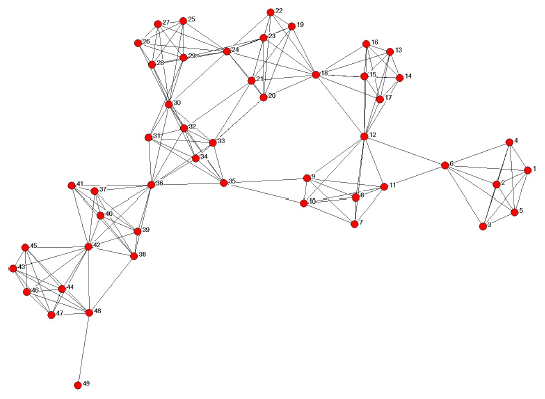
\includegraphics[width=11cm]{./imagenes/red_al_qaeda.png}
    \caption{Red social conformada por las células terroristas de Al-Qaeda.}
    \label{fig:red_al_quaeda}
  \end{center}
\end{figure}.

La evolución de los servicios proporcionados a través de la internet ha sido drástica puesto que ha cambiado el modo de vida de las personas. En la figura \ref{fig:utilizacion_internet} se evidencia que el crecimiento de la internet (de los servicios que en ella se soportan) se da en función de los servicios de conectividad social que son creados y soportados en ella. La web 1.0 fue utilizada en mayor medida por científicos para el intercambio de información en formato hipertexto. No había una interacción fuerte entre cada científico sino que ellos acudían a internet para buscar o poner a disposición material científico. Con la venida de la web 2.0 y la introducción de la interacción del usuario con la web, generando contenido en tiempo real, fueron creados servicios de redes sociales en-línea (OSN en inglés: On-line Social Network), produciento una partición en los tipos de redes sociales. Así, las redes sociales a las que pertenece el ser humano en la era digital se dividieron convenientemente en “redes sociales fuera de línea” y “redes sociales en línea” (Offline Social Network y Online Social Network)\cite[pag.3]{dynamics}.

\begin{figure}[!htb]
  \begin{center}
    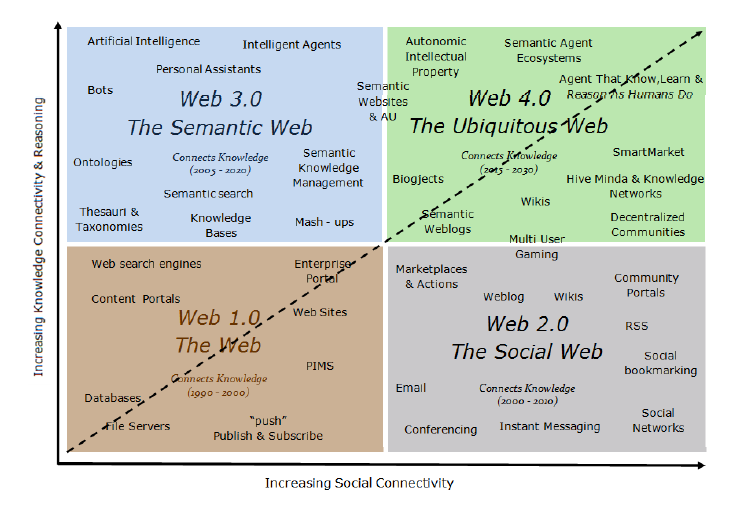
\includegraphics[width=11cm]{./imagenes/utilizacion_internet.png}
    \caption{Cambio de la utilización de internet en función de los servicios de conectividad social que son creados y soportados en ella}
    \label{fig:utilizacion_internet}
  \end{center}
\end{figure}

Las redes sociales fuera de línea son las redes sociales que se forman por comunicación tradicional (lenguaje oral y escrito en medios que difieran de aquellos que utilizan las telecomunicaciones). Las redes sociales en línea son aquellas redes sociales que están formadas por cibernautas y en las cuales la comunicación se da por medio de los servicios de redes sociales.\cite[pag.1]{analysis}

La administración de una red social fuera de línea fue estudiada desde inicios del siglo XX\cite[pag.3]{dynamics} con un enfoque socio-matemático llamado “análisis de redes sociales” (SNA por sus siglas en inglés: Social Network Analisis). Sin embargo, era difícil el análisis del comportamiento humano según los designios de la SNA, puesto que la información debía ser recopilada por medio de entrevistas a las personas. Aun así, el enfoque SNA fue utilizado para analizar el comportamiento terrorista o inclusive el comportamiento de trabajadores en una empresa.\cite[pag.6-13]{sna_startups}

Los estudios basados en SNA pueden ser de tipo egocéntrico o sociocéntrico\cite{user_behavior}. En los estudios egocéntricos de una red social, se analiza un individual dentro de una red social y todas las conexiones de éste hacia otros individuales en la red social analizada. El individual analizado es llamado “ego” y los individuales que hacen conexión con él son llamados “alters”. Se han identificado 4 capas en el estudio de las redes egocéntricas, estas son:

Support clique: En esta capa se identifican los alters con los que el ego hace más contacto por alguna razón de peso para él (e.g. para obtener soporte emocional). Esta capa tiene, en promedio, 5 alters.
Sympathy group: En promedio a éste corresponden 15 alters.
Affinity group: En promedio a éste corresponden 50 alters.
Active network: En promedio a éste corresponden 150 alters.

Los números dados en las capas descritas en el análisis egocéntrico son congruentes con el número de Dunbar, el cúal representa el umbral promedio de número de alters sobre la capa “active network” (150) según Robin Dunbar, argumentando que este límite se debe a la capacidad cognitiva del cerebro humano\cite[pag.3]{dynamics} (como más adelante será nombrado, los servicios de redes sociales ayudan al ser humano a gestionar su active network, proporcionando herramientas que, en teoría y de acuerdo a la brecha tecnológica, lo ayudarán a mantener sus lazos con los alters de su red ego).

El análisis egocéntrico permite conocer los factores que dirigen al ego a crear vinculos débiles o fuertes con potenciales alters, albergandolos en alguna de las cuatro capas o en ninguna.

Con la creación de las OSN y la gran cantidad de información que describe el comportamiento humano sobre este tipo de red social, ha sido más sencillo utilizar el enfoque de la SNA para estudiar que comportamientos tienen los humanos sobre una red social establecida.

Los servicios de redes sociales (SNS por sus siglas en ingles: Social Network Services) como Facebook, LinkedIn, Twitter, SportTracker o Xportia, ofrecen servicios para la gestión de la OSN de cada usuario que acceda a estas aplicaciones. Según un estudio hecho para medir la experiencia de usuario (UX por sus siglas en ingles: User eXperience) en los SNS, se encontraron 8 categorías que son críticas a la hora de diseñar una SNS y son:

\begin{enumerate}
  \item Self-expresion: Capacidad que tengan las OSN de compartir contenido relacionado a la vida real de los usuarios tal como lo pueden ser las fotos, los videos, los comentarios o las comunicaciones directas.
  \item Reciprocity: Interacción bilateral en tiempo real, es decir, interacción instantánea con uno o varios individuales en la OSN (por ejemplo, por medio de los servicios de mensajería instantánea).
  \item Learning: La información recibida por medio de la OSN debe poder ser utilizada en pro del desarrollo cognitivo del individual; debe existir información útil al individual que usa la OSN.
  \item Curiosity: El contenido de la OSN debe ser interesante para quien la utiliza.
  \item Suitability of functionality: Se refiere a cuán “utilizable” es una funcionalidad.
  \item Suitability of content: La calidad y exactitud de la información que en la OSN reside debe ser suficiente para el individual perteneciente a ella.
  \item Completeness of the user network: Los individuales deben querer pertenecer a la red social y buscar eficientemente a otros individuales para poder formar lazos con ellos y hacer crecer su red social.
  \item Trust and privacy: Confianza en los servicios de las OSN, así como también la capacidad que tiene el usuario de gestionar la privacidad del contenido que comparte en dicha OSN.\cite[pag.2-3]{social_experience}
\end{enumerate}

Cada uno de las categorías nombradas hace parte de los factores que impulsan la utilización de los SNS para la gestión de las OSN de las personas.

Un factor de éxito de la utilización masiva de las SNS es que éstas estén orientadas a un público en particular y aumenten su cobertura dependiendo de su alcance de masa crítica sobre una red social definida\cite[pag. PENDIENTE]{sna_startups}. Al construir, en principio, la red social deportiva enfocada en dos deportes en particular, DEPORTE 1 y DEPORTE 2, la probabilidad de ganar la masa crítica es mayor y, por tanto, el SNS desarrollado puede volverse más útil con el tiempo. Además de la especificidad del SNS en dos deportes, también se debe tener en cuenta a que población va dirigida. Según \cite{user_behavior_online}, entre los años de adolescencia y los 40 años de edad, las personas acuden con mayor interés al uso de los SNS; al ser la comunidad del deporte comprendida en su mayoría por personas entre la adolescencia y los 40 años, aumenta aún más la probabilidad de alcanzar la masa crítica y volver útil con el tiempo el SNS.

De acuerdo al enfoque SNA, las redes sociales pueden estar divididas en clusters, que no son más que agrupaciones de individuales sobre una red social por algún concepto como, por ejemplo, la pertenencia a una comunidad. Con lo anterior, podemos encontrar que algunos SNS ofrecen servicios para gestionar las OSN de sus usuarios centrándose en algún tipo de comunidad en específico y, la información que circula por ese tipo de comunidades, es diferente a la que pasa por SNS descentralizados (como Facebook y twitter). Viendo Facebook como una agrupación de clusters con temáticas diferentes (como lo son los deportes y la música, la ciencia y la vida cotidiana), se encuentran algunos SNS que enfocan sus servicios en alguna de estas temáticas. En este caso, el cluster o temática que compete al trabajo a elaborar es el deporte.

Se encuentra, entonces, otro de los factores que lleva a usuarios de SNS a utilizar los servicios que estas proveen de forma activa es la pertenencia de dichos usuarios a alguna comunidad (cluster) en particular\cite[pag.3]{dynamics}, así como también a la constante generación de información valiosa sobre la comunidad. 

Es posible hacer una división del cluster deporte en otros subclusters de cada uno de los deportes que existen en el mundo o en la clasificación de los deportes que han dado organizaciones como, por ejemplo, la IWGA (Internation WorldGames Association). Lo que se quiere con este trabajo es aportar al crecimiento de las redes sociales fuera de linea de las personas que practiquen deporte sin importar si lo hacen a nivel profesional o aficionado por medio de un SNS orientado a los deportes en general y, por lo tanto, el cluster que se ha escogido para trabajar es el del deporte como cluster mismo.

Otro factor en la creación de redes sociales (tanto fuera de línea como en línea) es la distancia entre cada individual y el posible tipo de enlace que los uniría. En \cite{evolution} se hizo un estudio acerca de la formación de lazos, la formación de triadas entre individuales de una red social basada en la inscripción localizaciones recomendadas y frecuentadas por los usuarios, teniendo como parámetros “la edad” o tiempo de vinculación del individual a la red social, el grado de cada individual (número de conexiones que tiene un individual a otro) y la localización de cada individual en la red social. También se analizó cómo afectaba la creación de nuevos lazos con la movilidad del usuario (el desplazamiento por lugares geográficos distintos). En conclusión, se verificó que la formación de lazos depende proporcionalmente de la edad y del grado del individual y es inversamente proporcional a la distancia que a cada individual y que la formación de lazos puede modelarse con solo dos de los tres factores (el grado y la distancia); en cuanto a la formación de triadas, se verificó que ésta depende de las características sociales de la red, tomando énfasis en los individuales compartidos entre los posibles individuales formadores de triadas. Además, en cuanto a la creación de nuevos lazos teniendo en cuenta los lugares visitados por cada usuario de la red social, se presenta un patrón: Los usuarios escogen un lugar popular para visitar y, posteriormente, dirimen con que usuario crear un lazo teniendo en cuenta su popularidad y que frecuente los mismos lugares siempre.

Al ver la importancia de manejar SNS que ofrezcan servicios de geolocalización, se ha visto pertinente añadir dicho servicio a la creación del prototipo de SNS orientado a los deportes en general.

Se investigó acerca de las redes sociales existentes enfocadas a la temática del deporte y se encontró que muchas de ellas son utilizadas en mayor medida en España y que todas ellas están soportadas sobre tecnologías web. En las tablas \ref{tab:comparacion_redes_1} a \ref{tab:comparacion_redes_4} se encuentra un análisis de las funcionalidades que presentan las redes sociales analizadas, así como también “que red social tiene que funcionalidad”. De acuerdo a lo expreso en las tablas, se ha escogido énfasis en las siguientes funcionalidades:

\begin{enumerate}
  \item Acceso a un repositorio de información acerca de los diferentes deportes soportados, de tal manera que el usuario pueda instruirse acerca de la indumentaria necesaria, reglas, historia, etc.
  \item Incluir información de salud para los diferentes deportistas, como rutinas de calentamiento, que hacer ante una lesión, etc. 
  \item Ubicar geográficamente los diferentes lugares, eventos y deportistas que practiquen un deporte de interés.
  \item Gestionar la creación y administración de eventos deportivos como lo son las ligas o torneos
\end{enumerate}

En general, solo se encontraron dos redes sociales deportivas orientadas a cualquier deporte asociadas a aplicaciones para smartphones disponibles en el la tienda virtual de Android o en la tienda virtual de Apple (La red social de Fitivity y Huddlers). Además, hay una ventaja real en hacer una red social orientada a dispositivos móviles y es la capacidad de movilidad que ellos brindan mientras se está utilizando el servicio\cite[pag.1]{spiderweb}. Dada la falta de aplicaciones móviles en el campo descrito y a su vez la importancia que toman los dispositivos móviles por sus características, se ha decidido hacer el prototipo de SNS orientado al deporte sobre tecnologías móviles y, más exactamente, tecnologías Android.

Así, con la evolución de la comunicación humana trasladándose a los espacios virtuales por medio de las OSN y la falta de aplicaciones, en el campo de los smartphones, que soporten interacciones sociales enfocadas a los deportes en general, en este trabajo se creará un SNS centrado en los deportes sobre tecnologías Android para la administración de las OSN de cada persona en un ámbito deportivo desde su dispositivo móvil.

